%!TEX root = ../main.tex

\section{Introduction}
Cryptography is the scientific field concerned with the study, development, and utilization of techniques aimed at secure communication between parties amidst the presence of adversarial entities seeking to intercept or manipulate transmitted data. In practice, it includes the creation and analysis of algorithms and protocols that aim to provide data confidentiality, data integrity, authentication, and non-repudiation. Modern cryptography is closely related to the fields of mathematics, computer science, and electrical engineering. Key concepts in this field include:
\begin{outline}
\1 Confidentiality, which ensures that only selected entities can access a set of information.

\1 Authentication, is the mechanism ensuring the genuineness of an entity's identity.

\1 Data Integrity, which verifies that data remains unaltered during transmission and detects any unauthorized modifications.
\end{outline}

A communication protocol is a definition of message formats and rules that are considered valid in communication. A protocol defines the syntax, semantics, and synchronization aspects of this communication. It stipulates the behavior of individual systems in an implementation-independent manner, allowing for protocols to be implemented in either hardware or software. For any successful communication, all participants must agree in advance on the protocols to be used.

A security protocol or cryptographic protocol protects communication using cryptographic methods. The fundamental services typically provided by cryptographic protocols are the authentication of participants, data integrity, and confidentiality, non-repudiation, and system availability (resilience to denial-of-service attacks). Alongside protocols directly protecting data, there exist protocols facilitating key exchange, negotiating communication parameters, and other auxiliary functions needed for establishing and maintaining secure communication.

Examples of cryptographic protocols include Transport Layer Security (TLS) which is used to secure HTTP traffic, the Diffie-Hellman key exchange which establishes a common secret over an insecure communication channel between two systems, and IPsec, which provides communication protection at the network layer of the TCP/IP stack.


\section{Cryptographic Algorithms}
Cryptographic algorithms serve as foundational elements in cryptography, offering essential mechanisms for secure systems. Due to their core position and heavy utilization in communication systems, attention to their efficiency is paramount.

There are various types of cryptographic algorithms, such as algorithms that provide data encryption, hashing, plausible deniability or deniable encryption, and steganography. Below we elaborate on the classes of cryptographic algorithms that are relevant to this thesis.


\subsection{Symmetric Cryptography}

Encryption is a transformation of a set of data into another, to secure this data from third-party access, i.e., aiming to provide confidentiality. The original data are called plaintext, while the data resulting from encryption are called ciphertext. The reverse transformation is called decryption.

Modern cryptography uses cryptographic keys for encryption and decryption, which parameterize the encryption algorithm. This parameterization decouples data confidentiality from cryptographic algorithm design. Assuming the algorithm is secure and implemented securely, then data confidentiality relies only on the secure protection of the key(s).

There are two basic types of encryption: symmetric and public key encryption. In symmetric encryption, a key is used for both encryption and decryption. The sender encrypts using the key, which is securely provided to the intended recipients, who in turn use it for decryption. Figure \ref{fig:figure2.1} illustrates the model of symmetric encryption.

% Figure 2.1
\begin{figure}[h!]
\centering
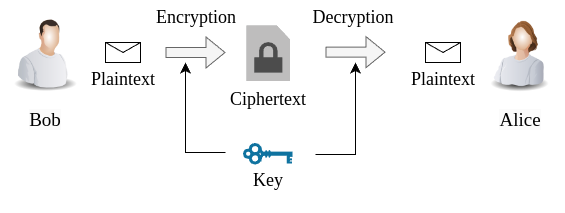
\includegraphics[width= 0.7\textwidth]{figure_2.1}\\
\caption{Symmetric Encryption}
\label{fig:figure2.1}
\end{figure}

% In symmetric encryption, two categories of algorithms prevail: block ciphers and stream ciphers. Block algorithms encrypt messages into equal-sized blocks, while stream algorithms encrypt bit by bit or byte by byte. The former are suitable when all data are available beforehand, whereas the latter encrypt data as it's generated (on-the-fly).

% For block algorithms, operation modes are crucial, detailing how the algorithm iterates over input data larger than the block size. When the input isn't a multiple of the block size, padding is employed to reach the appropriate size. The extended text is then inputted into the algorithm. Padding methods are typically specified in the algorithm's documentation. Various operation modes for block algorithms exist, including ECB, CBC, and CFB. Figure 2.2 illustrates CBC (Cipher-block Chaining).

Two categories of symmetric encryption algorithms exist, block ciphers and stream ciphers. Block ciphers encrypt a message into equal-sized blocks, while stream ciphers encrypt it bit by bit or byte by byte. The former are suitable when all data are available beforehand, whereas the latter encrypt data as it's generated (on-the-fly).

Block algorithms operate in modes that describe how the algorithm iterates over input data larger than the block size. When the input isn't a multiple of the block size, padding is employed to reach the appropriate size. The extended text is then inputted into the algorithm. Padding methods are typically specified in the algorithm's documentation. Various operation modes for block algorithms exist, including ECB, CBC, and CFB. Figure ~\ref{fig:figure2.2} illustrates the CBC (Cipher-block Chaining) mode \cite{rfc3602}.

% Figure 2.2
\begin{figure}[h!]
\centering
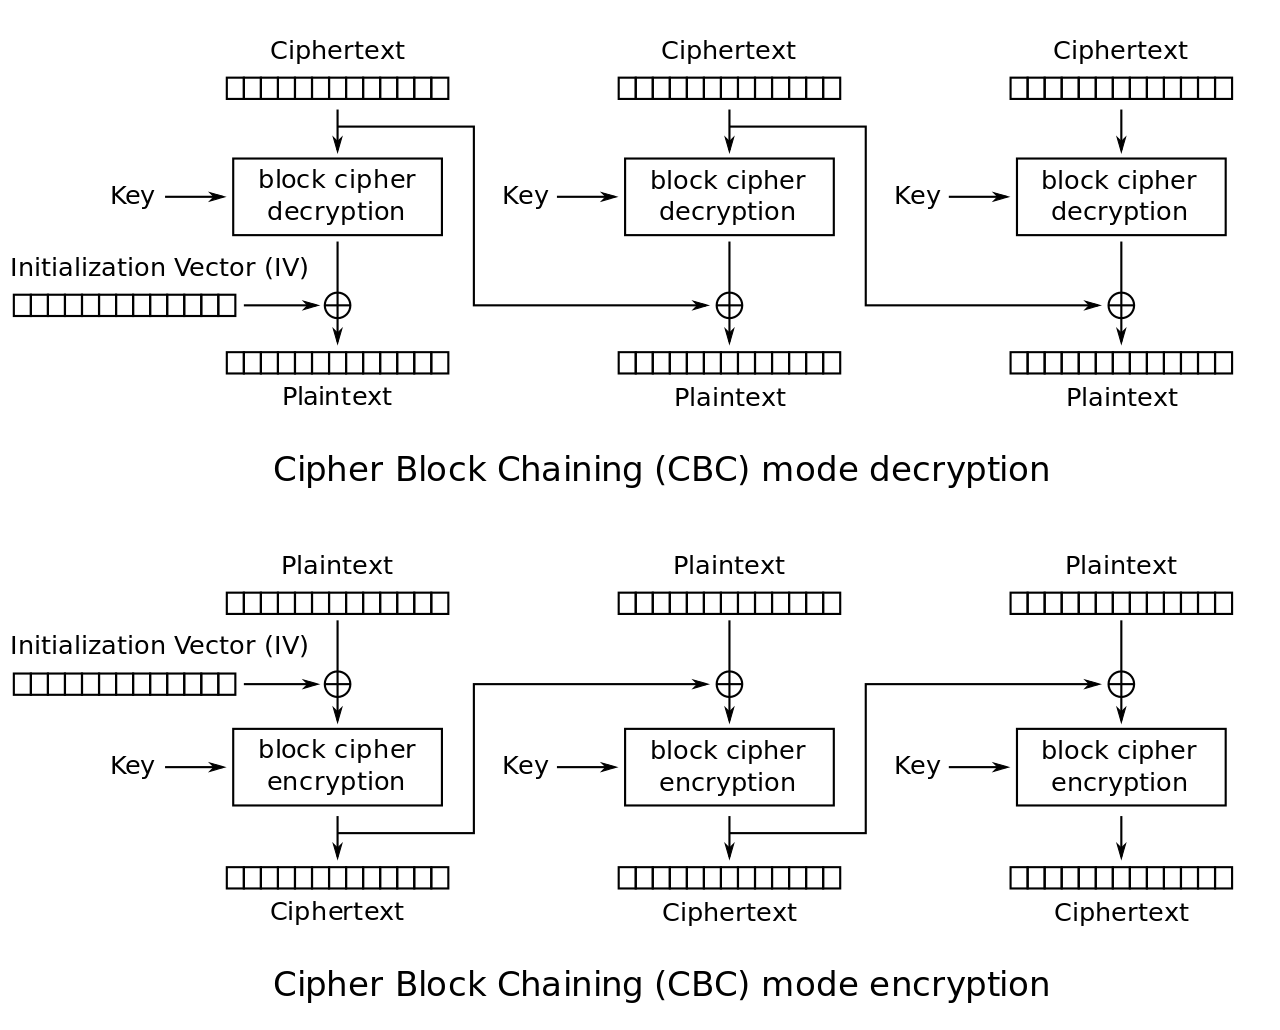
\includegraphics[width= 0.7\textwidth]{figure_2.2}\\
\caption{CBC Mode}
\label{fig:figure2.2}
\end{figure}

\newpage
\subsection{Public-Key Cryptography}
In public-key cryptography, each entity employs two keys: a public key and a private key. The public key is openly accessible, whereas the private key must be kept secret. These keys have the property that data encrypted with one key can be decrypted with the other. Furthermore, given the public key, discovering the private key is practically infeasible. Public-key algorithms serve two primary purposes: confidentiality and authentication.

When an entity wants to send information confidentially to another, it uses the other's public key to encrypt the data. Only the holder of the corresponding private key can access the plaintext. The process is illustrated in Figure ~\ref{fig:figure2.3}.

% fig 2.3
\begin{figure}[h!]
\centering
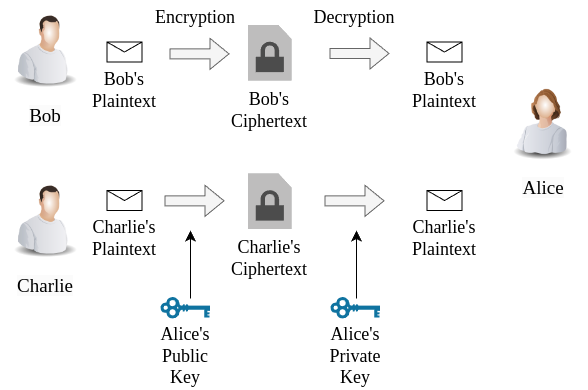
\includegraphics[width= 0.6\textwidth]{figure_2.3}\\
\caption{Public Key Encryption}
\label{fig:figure2.3}
\end{figure}

For authentication, the sender applies their private key to the data, generating a signature that is ideally impossible to forge.  Upon receipt, the recipient verifies the signature using the sender's public key. This process is illustrated in Figure ~\ref{fig:figure2.4}.


% fig 2.4
\begin{figure}
\centering
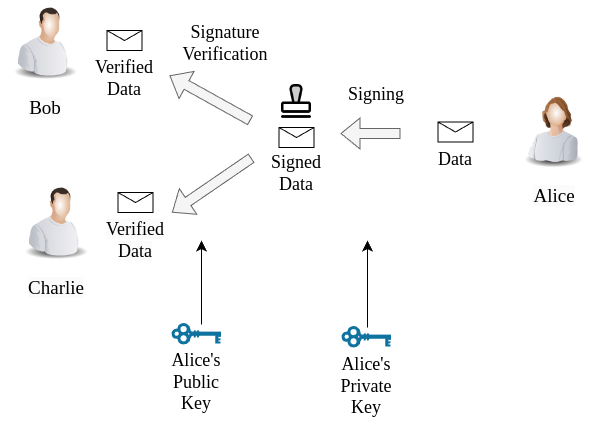
\includegraphics[width= 0.7\textwidth]{figure_2.4}\\
\caption{Public Key Signing}
\label{fig:figure2.4}
\end{figure}

Examples of applications of public key algorithms are digital certificates and secure key exchange (e.g., Diffie-Hellman) in TLS.



\subsection{Hash Functions}
A hash algorithm is a deterministic algorithm that maps variable-sized data to fixed-sized data, called hash or digest. Due to the finite number of potential outputs compared to the infinite input space, hash algorithms inevitably encounter collisions, where distinct inputs yield identical outputs.


% fig 2.5
% \begin{figure}
% \centering
% \includegraphics[width= 0.7\textwidth]{figure_2.5}\\
% \caption{}
% \label{fig:figure2.5}
% \end{figure}

In cryptographic applications, cryptographic hash functions adhere to additional stringent criteria:
\begin{outline}
\1 Difficulty in finding an input that generates a specific output.
\1 Difficulty in modifying the input while keeping the output the same.
\1 Difficulty in discovering two inputs that produce identical outputs.
\end{outline}

The higher the degree of the above difficulties, the greater the hash algorithm's security. Cryptographic hash algorithms primarily serve serve data authentication and integrity purposes. Notable examples include MD5, RIPEMD, and SHA \cite{fips_118_2}.


\subsection{Keyed Hash Functions}
To ensure data integrity and authentication, message authentication codes (MACs) are commonly employed. A MAC consists of a small piece of information appended to the message to enable verification upon receipt. Cryptographic hash algorithms are often used in conjunction with a key (Hash-based MAC – HMAC) which is accessible solely to the communicating endpoints. Any cryptographic hash algorithm, such as SHA-1 and MD5, can compute an HMAC, resulting in algorithms like HMAC-MD5 and HMAC-SHA-1, respectively. The process is depicted in Figure \ref{fig:figure2.6}.

% fig 2.6
\begin{figure}
\centering
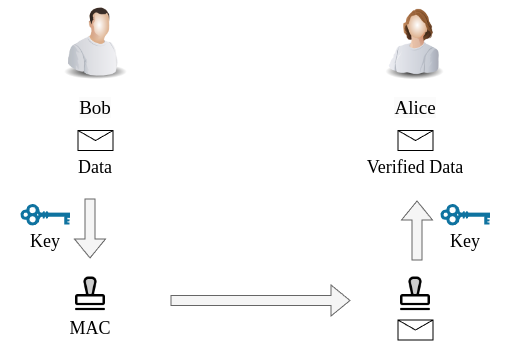
\includegraphics[width= 0.6\textwidth]{figure_2.6}\\
\caption{HMAC Operation}
\label{fig:figure2.6}
\end{figure}

\subsection{Pseudorandom Number Generators}
Random Number Generators (RNGs) are algorithms designed to generate sequences of numbers that mimic randomness. Two categories of RNGs are True RNGs and Pseudo RNGs.  True RNGs are generators that usually generate numbers from random physical phenomena while Pseudo RNGs usually rely on a small amount of physical randomness, called seed, which they use to further generate numbers that appear random but are not truly random as they still exhibit patterns and repetitions. 

In cryptography, RNGs play a vital role when randomness is required for security. They are commonly utilized in tasks such as cryptographic key generation and initialization vector creation.

\section{Key Management}
Key management encompasses key creation, distribution/exchange, storage, and replacement—a crucial process for system security often challenging to implement due to policy considerations and external factors.

Before initiating secure communication, entities must establish communication parameters, including cryptographic keys for symmetric encryption. Key exchange facilicates the need to establish such keys over insecure communication channels. A notable key exchange protocol is the Diffie-Hellman exchange.

Keys undergo a lifecycle, necessitating periodic replacement. This practice mitigates risks associated with key compromise. Regular replacement limits the impact of key exposure and adds complexity for malicious entities, as it reduces the volume of data encrypted with a single key, thereby limiting available data for cryptanalysis.

\section{Security Hardening}
Several considerations are involved when trying to improve the security of a cryptographic system. One of the most important parameters in security is the key size. It directly correlates with security strength; larger sizes correspond to increased security levels. Furthermore, encryption algorithms are evaluated based on the important properties of confusion and diffusion. Cryptographic hash algorithms should exhibit collision resistance, making collisions difficult to find. Similarly, an effective pseudorandom number generator should produce sequences with extended periods before repetition. Beyond these algorithmic properties, additional techniques are employed to bolster security at the implementation level, such as side-channel countermeasures and formal verification techniques.


\subsection{Padding}
In addition to configuring appropriate input sizes for block algorithms, data extension also helps conceal the actual size of the data packet. Additional padding can be used as a way to increase security albeit at the cost of throughput.


\subsection{Salt}
The term "salt" is used to denote additional data added to the input of hash algorithms. Adding salt to the input results in a different output from the algorithm, even with the same input. This method mitigates attacks such as rainbow tables.


\subsection{Initialization Vectors}
An Initialization Vector (IV) is random data the size of a block which is placed at the beginning of the plaintext data, with the aim of further enhancing the security of block algorithms. They introduce randomness into the encryption process since for encrypting the same text under the same key, the result will depend on the IV value. The requirement for IVs is that they need to be unpredictable.






